 \documentclass[12pt]{article}
\usepackage{mathtools}
\usepackage[margin=1.3in]{geometry}
\usepackage{graphicx}
\usepackage{amssymb}
\usepackage[colorlinks]{hyperref}
\usepackage{textcomp}
\usepackage{courier}
\usepackage{textgreek}
\usepackage[font=small,labelfont=bf]{caption}
\usepackage{tabularx}
\usepackage{subcaption}
\usepackage{float}
\usepackage{fancyvrb}

\usepackage{fvextra}
\usepackage[breaklinks=true]{hyperref}
\usepackage{breakcites}
\usepackage{subcaption}
%\graphicspath{{graphics/}}
\setlength\parindent{0pt}

\begin{document}

\begin{titlepage}
    \begin{center}
        \vspace*{1cm}
        
        \Huge
        \textbf{Automatic evaluation of liver cirrhosis in lung cancer patients receiving radiotherapy}

        \vspace{1.5cm}
        
        \LARGE
        \textbf{Gabriel Battcock}\\
        \textbf{9618026}
        
        \vfill
        
        Second semester report
        
        \vspace{0.8cm}
        
        
\includegraphics[width=0.2\textwidth]{graphics/UomCrest.jpg}\\
        \large
        MPhys project\\
        School of Physics and Astronomy\\
        The University of Manchester\\
        May 2020
        
    \end{center}

\end{titlepage}

\thispagestyle{empty}
    \begin{center}
        \Large
        \textbf{Automatic evaluation of liver cirrhosis in lung cancer patients receiving radiotherapy}
        
        \large
        \vspace{0.4cm}
        \textbf{Gabriel Battcock}
    \end{center}
    

\begin{abstract}
\noindent
In the treatment of lung cancer, computed tomography (CT) scans are used routinely to identify tumours.  As the data from CT scans can be used in a non-invasive way to identify liver cirrhosis, a link between the two diseases and the treatment of lung cancer can be investigated. The study used an automated process to identify patients’ livers on CT scan images and trained a transfer learning neural network to perform automated segmentations of the liver.  The data from the original scan and the automated segmentations was analysed using contouring algorithms to compare the surface of the sampled liver with the smooth surface of a supposed healthy liver. This returned a liver surface nodularity (LSN) score, a biomarker for liver cirrhosis. There was a clustering of values below a score of 1.46 which could indicate that cirrhosis may be present above this value, but clinical data is needed to support this. Comparing LSN values for automatic segmentation with manual segmentation, it can be concluded that segmentation using a neural network is a valid approach. Further work in this area is needed to fully automate the system, leading to research into cirrhosis as a potential biomarker for the treatment and survival of lung cancer. 
\end{abstract}

\newpage

\section{Introduction} 
The aim of this study was to assess a technique to automate the analysis of liver cirrhosis using computed tomography (CT) scans.  %This would enable large data sets to be studied effectively and could be used to study the effects of liver cirrhosis on how well a patient responds to treatment for lung cancer, and ultimately to survival.
Radiotherapy treatment for lung cancer induces an immune response, and the liver is important to the immune system  \cite{Wang:2018aa} \cite{Kubes:2018aa}. Therefore, the health of other organs such as the liver could be used as a biomarker of how well the patient is responding to the treatment. The level of cirrhosis of the liver is an indication of the health of the liver. Cirrhosis analysis using CT scans is a relatively recent technique that involves a manual input from a doctor. Automating the system would enable large data sets to be studied effectively. Looking for a relationship between liver cirrhosis and its effect on the immune system and thus to survival will be valuable.  This can be achieved by creating an automated system to evaluate liver cirrhosis so further research can be performed in this area.  
\\ \\
To investigate the aim, three main steps were proposed. The first, to use a programme to automatically find a slice of liver from the full CT scan; the second to use a pre-trained transfer learning neural network to automatically segment the liver; and third to create a programme that analyses the liver and calculates an LSN score.
\\ \\
Sections were shared between Gabriel Battcock and Theodore Cohen. Theodore Cohen worked on the first section and the neural network, and Gabriel Battcock worked on the first section and the LSN score.

\subsection{Liver cirrhosis}
Scar tissue is created in the liver as it heals itself from damage. A build up this tissue is known as liver cirrhosis. Cirrhosis can cause many problems including portal hypertension, jaundice and enlargement of the spleen \cite{mayo_clinic}. 
\\ \\
As liver cirrhosis is best diagnosed using an invasive biopsy, the number and size of samples are kept to a minimum \cite{Huang:2007aa}. This poses a number of risks in respect to sampling errors and biased results arising from small samples of liver being taken \cite{Huber:2015aa}. Other non-invasive tests have been created like liver-stiffness measurements but have disadvantages that make them undesirable \cite{Smith:2016aa}. 
\\ \\
A recent development in diagnosis is the use of computer programmes to look for biomarkers of cirrhosis from CT scans. By evaluating the roughness of the surface of the liver compared to the surface of a healthy, smooth liver, a liver surface nodularity (LSN) score can be obtained. This is an important biomarker for liver cirrhosis. The LSN score can \textit{"accurately differentiate cirrhotic from noncirrhotic livers
and is highly reproducible"} (A D Smith et al.) \cite{Smith:2016aa}. With this method, a region of interest (ROI) is selected by doctor, and the programme automatically draws a polynomial line for where the surface should be and a line for its true surface.  

\subsection{CT Scans as data}
CT scans are used widely in hospitals to image sections of the body. Many 2D image slices of the body are stacked together to create a 3D image of the body. Different tissues in the body are represented as different shades of grey, proportional to how much radiation they absorb. This makes internal organs appear distinct \cite{Broder:2011aa}.  
\\ \\
CT scans are used to diagnose various diseases including cancers, heart disease and head injuries. In this study, lung cancer patients were studied. After lung cancer has been diagnosed and the patients are receiving treatment, the patient undergoes a CT scan, taken from the top of the torso to below the lung. The data from the CT scan is used to locate tumours for treatment using radiotherapy, and to track the change in their size \cite{Purandare:2015aa}. There is a wealth of data from lung cancer patients that can be used to investigate other diseases that may be present in patients who have lung cancer. %maybe look at rewording this
\\ \\
Directly below the lung in the human body is the liver (Figure \ref{lung_and_liver}). Scans of lung cancer patients include the liver. Using the large cohort of previous patients, one can investigate a connection between the health of the lungs and the health of the liver in terms of treatment and ultimately survival.
\\ \\
\begin{figure}[htp]
    \centering
    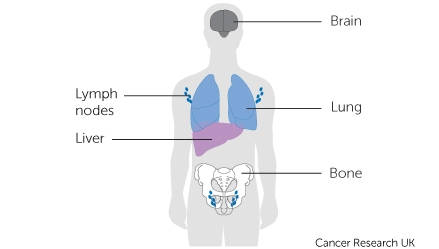
\includegraphics[width=\textwidth]{graphics/lung_and_liver}
    \caption{Visual of organs in the body, showing that the liver is located directly below the lungs, taken from Cancer Research UK \cite{body_diagram}.}
    \label{lung_and_liver}
\end{figure}

 

\section{Theory}
\subsection{CT scans}

\color{black}
CT scans use X-rays to take many image slices of the body. These CT slices can vary in thickness from \hbox{1-10 mm}. Images of the CT slices are saved as digital imaging and communication in medicine (DICOM) files. Each file includes a header file which includes important metadata, such as patient ID, slice location, slice thickness and other information about the patient and the scan \cite{Varma:2012aa}. Many CT slices are taken for each patient and saved in a CT scan folder.
\\ \\

 Each pixel in of a CT scan slice has a value given in a dimensionless unit called the Hounsfield Unit (HU). This is defined on \hbox{-1000 HU} for air and \hbox{0 HU} as distilled water \cite{hounsfield}. Thus, values for other tissue and body parts can be found using:
\begin{center}
\begin{equation}
   HU=\frac{\mu_X-\mu_{water}}{\mu_{water}-\mu_{air}}\times1000
   \label{hounsfield_equation}
\end{equation}
\end{center}

where $\mu_i$ is the linear attenuation coefficient, a measure of how easily a material can be penetrated by radiation \cite{Lamba:2014aa}. 
\\ \\
%Typical values of internal organs can be seen in Tab. \ref{HUorgans}. The liver and fat have distinct values and thus can be distinguished from each other well.

%\begin{table}[h]

 %   \centering
 %   \caption {Table listing HU values for various organs and material that are in close proximity to the liver \cite{Lamba:2014aa} \cite{Broder:2011ab}.}
 %   \label{HUorgans}
  %  \begin{tabular}{c|c}
  %      Organ & HU value\\
  %      \hline
  %      Liver & 50.4 \\
  %      Midline anterior subcutaneous fat & −113.4 \\
  %      Lung & -498 \\
  %      Bone & 570 \\
  %      Soft tissue & 56 \\
  %      
  %  \end{tabular}

%\end{table}

To convert from HU values to grey scale, on range [0,255], a process called windowing is used. This is composed of two parameters; window-width and window-level. Window-width refers to the how large the range of values that are converted to grey scale is. A window can be wide or narrow depending on the organ or tissue being examined \cite{window_level} \cite{Xue:2012aa}. Window-level is the midpoint of the window range being displayed. Changing these values together can highlight features of the scan that are not immediately apparent, as seen in Figure \ref{window_level_figure}.

\begin{figure}[htp]

\centering
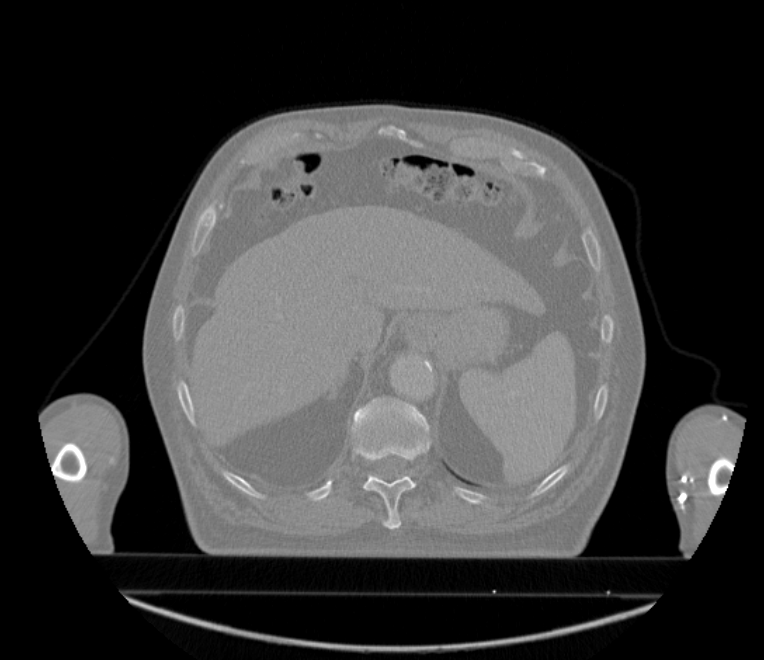
\includegraphics[width=.3\textwidth]{graphics/window_level_orig.png}\hfill
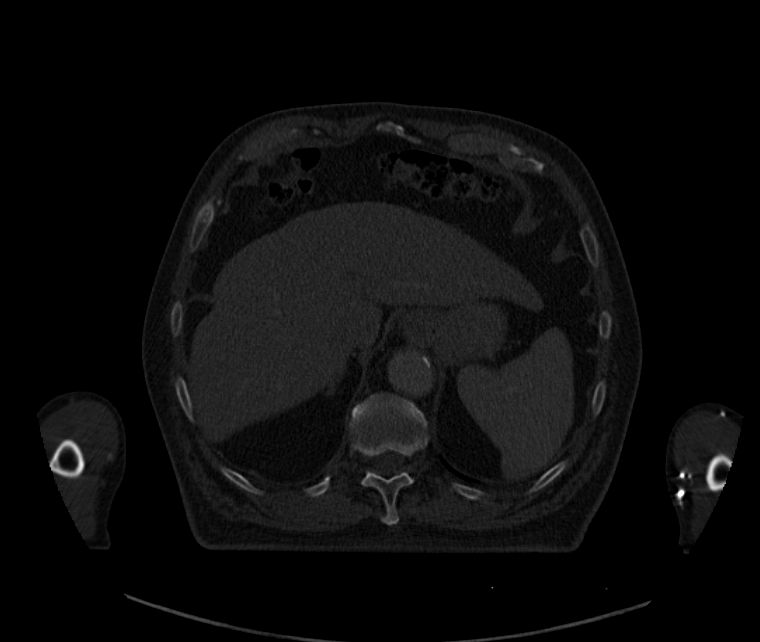
\includegraphics[width=.3\textwidth]{graphics/level_change.png}\hfill
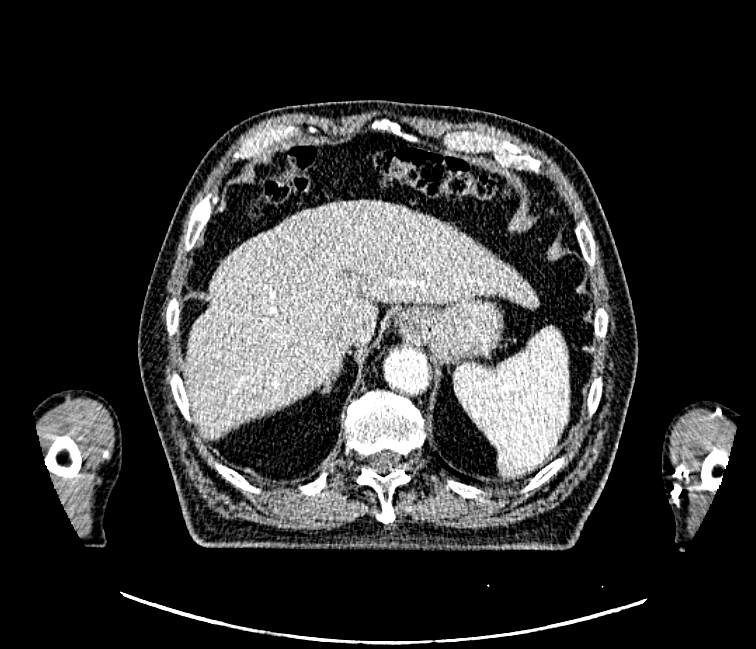
\includegraphics[width=.3\textwidth]{graphics/window_change.png}

\caption{These images show three different windowing settings for the same image. The image on the left is the original, showing the liver and fat that look similar in terms of grey scale. The middle image has a higher window-level value. The right image is of the liver with a narrower window-width. In this image, there is a very obvious boundary between the fat and the liver that is not as clear in the original.}
\label{window_level_figure}
\end{figure}


\subsection{Liver segmentation }
\label{lsn}
%\color{red}
%Talk about where a good section of the liver to use is and why (bit next to fat for good contrast). Not wanting a slice on inside due to the slope. 
%\color{black}
The first step in the process of liver segmentation is finding a suitable CT slice of the liver to segment. To do this automatically, a programme has to recognise the liver from a full CT scan. An ideal slice of the liver is one which has a border with fat, as it has a good contrast giving a clear liver surface. Only the outer boundary of the liver was chosen due to well defined surface surface. Slices that contain gas, such as the bottom of the lung or bowl gas is best to be avoided. This is useful for training a neural network and for calculating an LSN score. To find this, the programme would try to identify for the middle of the liver. 
\\ \\ 
%\color{red}
%Discuss what the LSN score is and how(?) it is calculated. Give examples from other papers about what a good/bad score would be. 
%\color{black}
To make a quantitative assessment on liver cirrhosis based on a CT scan, a metric called the liver surface nodularity (LSN) score is used. As the liver builds up more scar tissue, the liver surface becomes wrinkled, a symptom known as fibrosis \cite{Wynn:2008aa}. This textured surface can be detected by on a CT scan. An LSN score can be calculated by finding the mean distance between two lines drawn on the boundary of the liver (the first is a smooth polynomial line for where the boundary of a healthy liver would be; the second is the detected edge of the liver, calculated using active snake contours). The LSN score is defined as the mean pixel-by-pixel distance between the polynomial line and the detected boundary \cite{Smith:2016aa} \cite{Sartoris:2018aa} \cite{Kim:2019aa}.  Through analysis of an LSN score distribution based on clinical data, an assessment of what stage of fibrosis a patient is at, with stage 4 fibrosis being cirrhosis \cite{Schuppan:2008aa}. Using this definition, a higher LSN value would indicate a liver that is more likely to be cirrhotic. 
\\ \\
%\color{red}
%Discuss the how active snake contours and geodesic active contours are determined. 
%\color{black}
To find the two boundaries of the liver previously outlined, active contour algorithms are used. These models are used to accurately describe the boundaries of objects in images, and can be manipulated for the purposes of detecting the liver surface from a CT scan. In image processing, energy is a way of measuring the uniformity of an image. Active contour algorithms work by finding the minimum energy of the line (in terms of mechanical energy of stress and strain), with external constraints of the energy of the image that guide it towards boundaries \cite{Kass:1988aa}. As explained in Kass et al., the energy functional of the snake, $E^*_{\mathrm{snake}}$ is:
% https://stackoverflow.com/questions/4562801/what-is-energy-in-image-processing 
\begin{equation}
    \centering
    {E^*_{\mathrm{snake}}}= \int^1_0E_{\mathrm{int}}(\boldsymbol{v}(s))+ E_{\mathrm{image}}(\boldsymbol{v}(s))+E_{\mathrm{con}}(\boldsymbol{v}(s)) ds
\end{equation}

where $E_{\mathrm{int}}$ is the internal energy of the line, $E_{\mathrm{image}}$ is the energy of the image, $E_{\mathrm{con}}$ is the energy of the constraints and $\boldsymbol{v}(s)$ is the parametric equation for the snake. The energy of the image consists of energy of lines and edges. Thus, finding the minimum of this functional, given appropriate parameters, will find the boundary of the given image. These parameters include starting boundary conditions for the snake, smoothness and attraction to edges. 
\\ \\
Another way to to find the boundary on images is by using morphological active contours. These are similar to the active contour, but have a better stability for grey scale images \cite{Marquez-Neila:2014aa}.

\subsection{Neural network}
%\color{red}
%Talk a little bit about transfer learning neural networks, but only enough to explain why they were used.
\color{black}
Machine learning is a process in which a computer learns how to complete a task through systematised trial and error. The use of supervised machine learning gives the computer a set of inputs and outputs which then optimises a way of connecting the two together using a layers of nodes \cite{Sabharwal:2011aa}. Two methods of training network exist: supervised learning where the network is given labelled inputs and outputs to map to each other; and unsupervised, where the network is not given the output and looks for patterns in the input data \cite{Chollet:2018aa}.
\\ \\
Networks are trained by minimising a loss function. A loss function is a method of comparing the true output with the output of the training network. The Dice-Sorensen coefficient is a measure of how similar the input and output are, as given by
\begin{equation}
\centering
\mathrm{DSC}={\frac{2\vert{A\cap B}\vert{}}{\vert{A}\vert{}+\vert{B}\vert{}}},
\end{equation}
where $A$ and $B$ represent the true output values and the output of the training network \cite{Dice:1945aa}. The network tries to minimise the loss function, defined as as \hbox{1-DSC}. This is achieved through calculation of the negative gradient of the loss function 

\begin{equation}
\centering
{-\nabla L}={\sum_{i=1}^n \frac{\partial L}{\partial w_i}\cdot \mathbf{w_i}},
\end{equation}
where $L$ is the loss function and $w_i$ are the weights of each node. The neural network iterates this process until the loss function has been suitably minimised, with the resulting weights forming a trained network which can be used to solve the problem initially set.

\section{Method}
\subsection{Identifying the liver from full CT scans}

To investigate liver cirrhosis in lung cancer patients, an open source data set of lung cancer patients from the Cancer Imaging Archive was used \cite{dataset}. This included CT scans of 422 patients, of which a sample of 100 was used for the analysis. The data was input into a Python file and manipulated using the PyDICOM package \cite{Mason:2011aa}.
\\ \\
Two methods of finding a suitable slice of the liver from a full CT scan were proposed. The first method was to find the liver using the mean pixel value of slice against the position in the body to find where the lungs ended, and thus the liver. This method using mean pixel value was discussed after reviewing slices of the whole CT scan. Lungs appear dark due to their composition of mostly air, whereas the liver is bright and large.
\\ \\
The second method was to use connected components to find the bottom of the lung and thus the liver. Connected components in image processing is a method of labelling sections by first creating a binary image using a threshold value, below which pixel will be zero and above will be one. Pixels of the same that share an edge or corner are considered to be connected. This can be transferred to 3D when taking into by treating voxels that border in the same manner. By applying this to a full CT scan, the lungs were found as the second largest connected component. Using the bottom of the lung as a marker for where the liver is, slices were found. 
\\ \\
Once a suitable slice of the liver was found for a patient, a manual segmentation was performed using the package Slicer \cite{slicer}. A painting tool was used to highlight the boundary of the liver. The segmentation images were saved as a binary Nifti (Neuroimaging Informatics Technology Initiative) file, as a 3D array. These were converted to a 2D Numpy (npy) array using Nibabel package \cite{nibabel}. Files of the binary map and original slice were saved together as npy files, to be used for training the neural network and for  drawing a smooth polynomial line on the boundary of the liver.

\subsection{Neural network}
To automatically segment the liver, a transfer learning convolutional neural network (CNN) written by Dr Andrew Green was used. This was previously used to segment muscles in work on sarcopenia \cite{Green:2019aa}. The network used a UNet like architecture which works with fewer training data than typical neural networks need \cite{2015arXiv150504597R}.
\\ \\
The network can be used for coloured images so has three input channels for red, green and blue (RGB). Images were formatted with different windowing settings to act as different colours. Augmentation was used to generate more training data through a combination of rotations and zooms. The top layers of the network were trained for ten epochs after which the whole network was trained. A reduced learning rate was implemented and the network would stop early if suitable weights were found before the entire cycle had run. 61 segmentations were used in the training set, with five in validation and six in the test set. 


\subsection{Calculating the LSN score}
To calculate the LSN score, two lines were drawn on the boundary of the liver, as described in Section \ref{lsn}. To handle the data, a class was created for the patient which included the binary mask file and the original CT image of the liver. Within this, functions were created for finding the smooth polynomial line and the true boundary of the liver.
\\ \\
To find the true boundary of the liver, a geodesic active contour (GAC) was used on the CT image. The background of the image was removed using a threshold to set dark pixel to not a number (NaN) so it would not interfere with the contouring. For the GAC to find the minima of the image, the slice had to be preprocessed into the form of an inverse Gaussian gradient. This applies a Gaussian filter to blur the image and then take the inverse of the first derivative of the image. The resulting array has areas of local uniformity around one and areas close to a boundary as close to zero \cite{inverse_gaussian}.
\\ \\
The contour algorithm works by using an initial line which then expands or contracts to find the minimum value from the input parameters. For the boundary of the liver, the initial contour was a small circle set in the centre of the liver. A threshold value between HU values for the liver and fat was set so that the initial contour, after expanding from the centre (ballooning), would converge toward, marking out the boundary of the liver.


\section{Results}
\subsection{Identifying the liver from full CT scans}

In the investigation of trying to identify the liver from a full CT scan, two methods were performed. Using the CT scan data in a Python file, the first method for finding a slice of the liver was tried. Plotting the mean pixel value against the slice position, clear maxima and minima were found (Figure \ref{fig:1}). These maxima corresponded to a region inside of the liver. However, it was not always a slice with a clear boundary with fat that could be used for LSN analysis. Figure \ref{mean_pixel_value} shows the findings of the initial approach. After looking through for the maximum mean pixel slices for patients in the data set, the programme would sometimes return a CT slice of the shoulder blades, due to bone being thick in this region while also having a high HU value. To solve this problem, the first \hbox{10 cm} of the CT scan was not be included.
This is valid for CT scans of lung cancer patients as removing \hbox{10 cm} from the top of the scan will only remove shoulder blades or the top of the lung and will not affect the slices of the liver. 
\\ \\
\begin{figure}
  \centering
  \subfloat[]{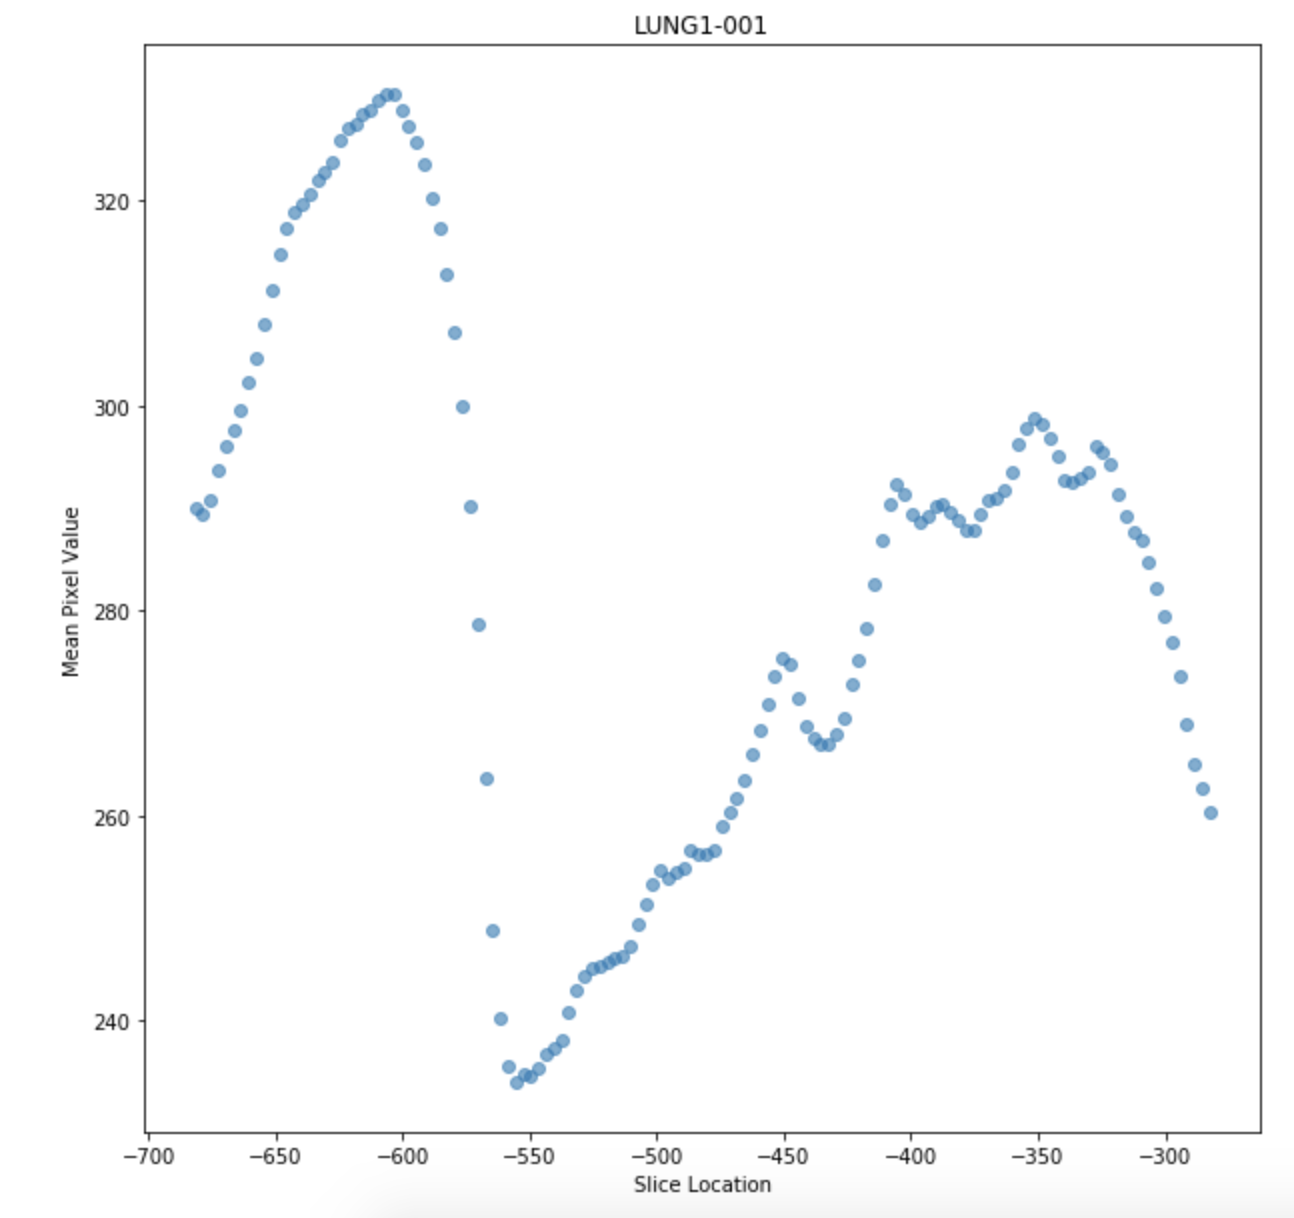
\includegraphics[width=.65\linewidth]{graphics/mean_pix_1.png}\label{fig:1}}

  \subfloat[]{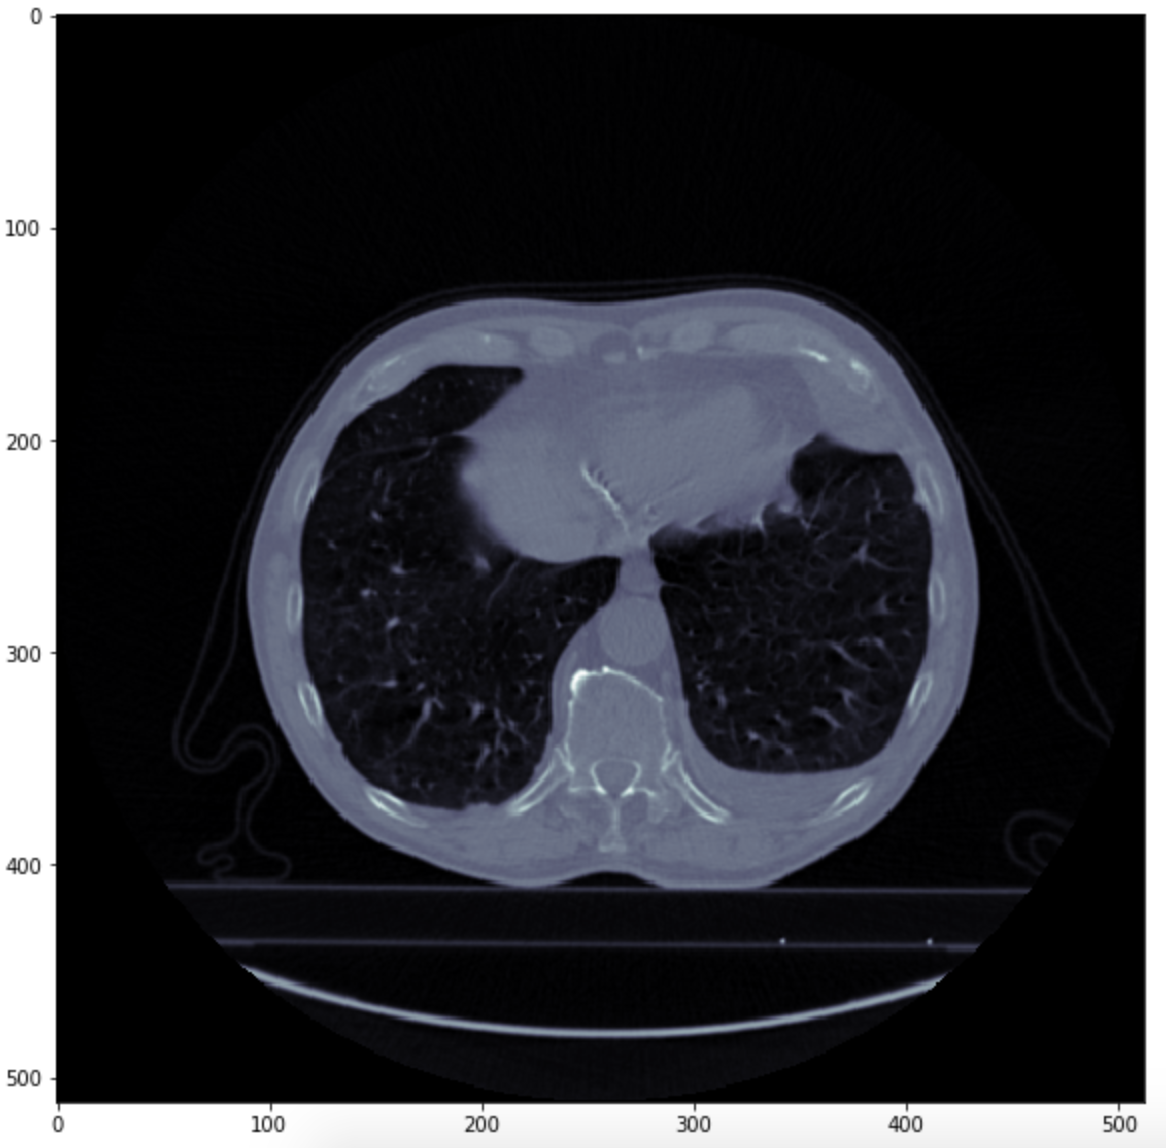
\includegraphics[width=.4\linewidth]{graphics/mean_pix_3.png}\label{fig:2}}\hspace{1em}
  \subfloat[]{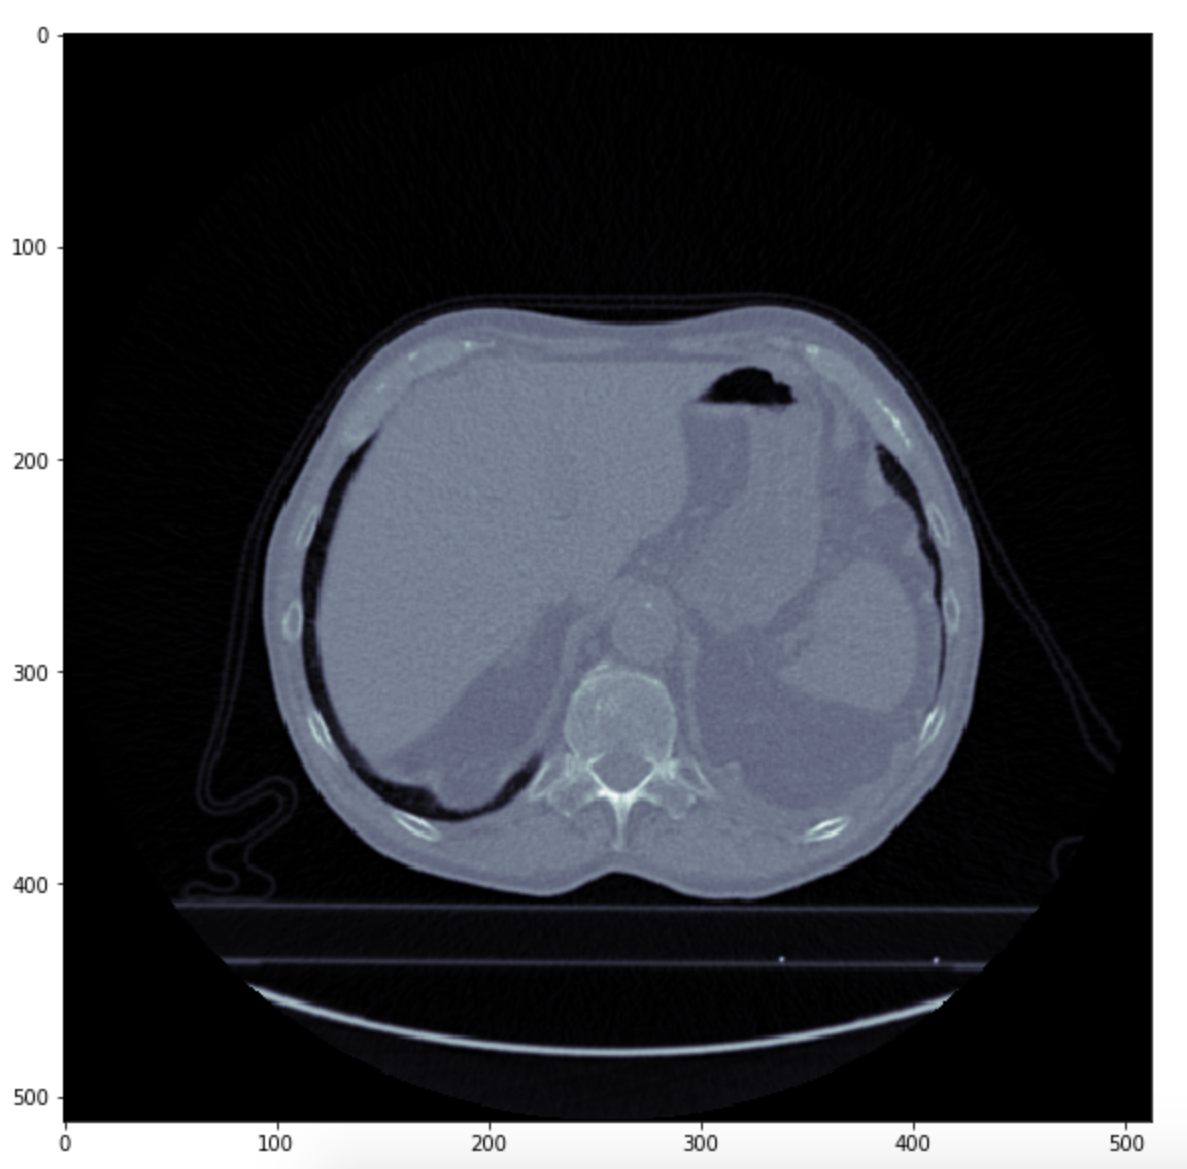
\includegraphics[width=.4\linewidth]{graphics/section3.1max.png}\label{fig:3}}
  \caption{Findings of the liver from a patient's full CT scan using the mean pixel value. Figure \ref{fig:1} shows a plot of the normalised mean pixel value against the slice location. The global minimum and global maximum are Figure \ref{fig:2} and Figure \ref{fig:3} respectively. Figure \ref{fig:2} shows the middle of the lungs, while Figure \ref{fig:3} shows a slice of the liver. }
  \label{mean_pixel_value}
\end{figure}

Due to the first method not consistently finding suitable slices of the liver with a clear boundary with fat, the second method was performed using connected components. However, this had the same problem as the first approach, not consistently identifying a suitable slice that could be used for segmentation. This was due to variability in the shape of the lung and the shape of the liver. Lungs can extend low into the torso, resulting in a slice of the liver that is too low down. A technique of blurring and redefining was used to avoid this by making the bottom lungs appear more smooth. However, this would sometimes end up with a CT slice of the liver that borders the lung, which is not ideal for segmentation. All bodies are different, so finding a consistent section of the liver is not always possible.


\subsection{Transfer learning neural network}

%Discuss very briefly what numbers were used and what the results are.
%Don't really know what to discuss here. What optimizing functions were used, what value of loss we get, show some results of the segmentation. 
\color{black}
The convolutional neural network described in the method was applied to the training data set and tested on the test set. The evolution of the loss function for the neural network can be seen in Figure \ref{fig:loss_function}. An average minimum loss function of the DSC for the test set of six CT scans was \hbox{$0.0032\pm0.0018$}. For the six test scans, the individual DSC values can be seen in Table \ref{tab:comparison}. An example of a manual segmentation next to the output of the CNN can be seen in Figure \ref{fig:Segmentations}.

\begin{figure}[htp]
    \centering
    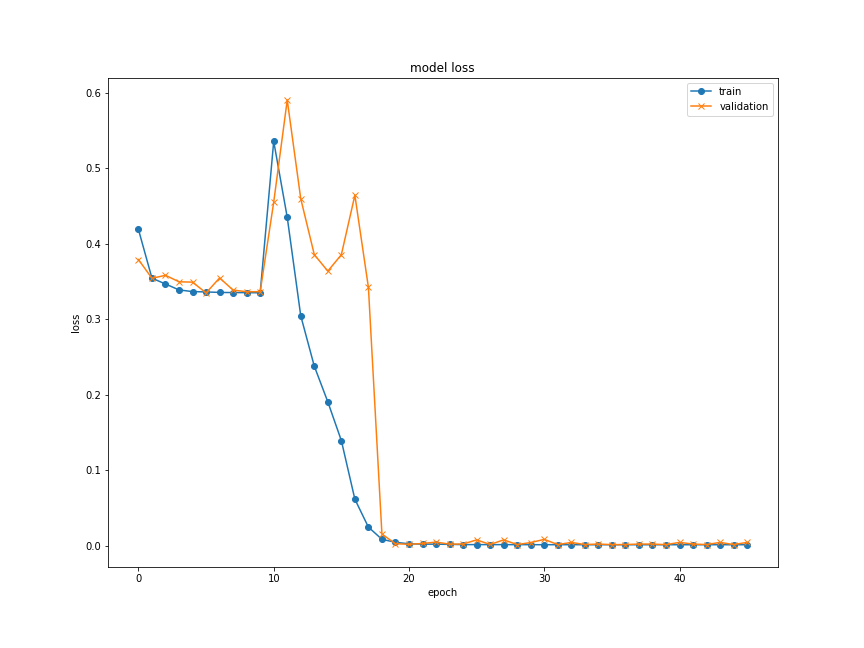
\includegraphics[width=0.8\linewidth]{graphics/LossGraph.png}
    \caption{Plot showing the evolution of the loss function against the number of epochs. A minimum value is seen at 0.0032.}
    \label{fig:loss_function}
\end{figure}

\begin{figure}[h!!]
  \centering
  \subfloat[]{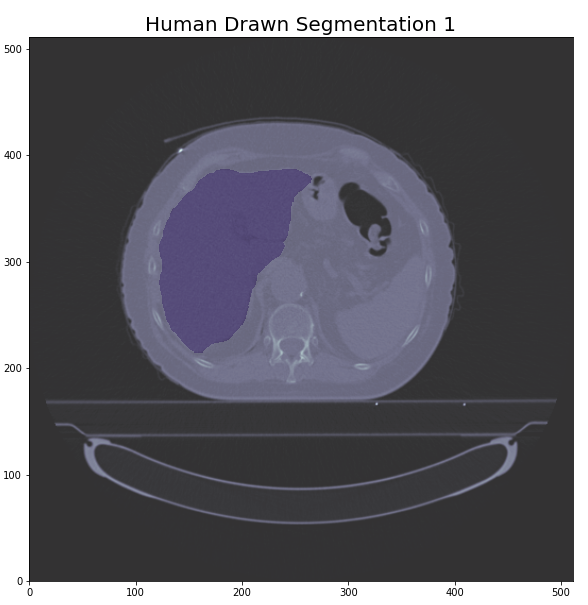
\includegraphics[width=.4\linewidth]{graphics/HumanDrawnSegmentation0.png}\label{Human}}\hspace{1em}
  \subfloat[]{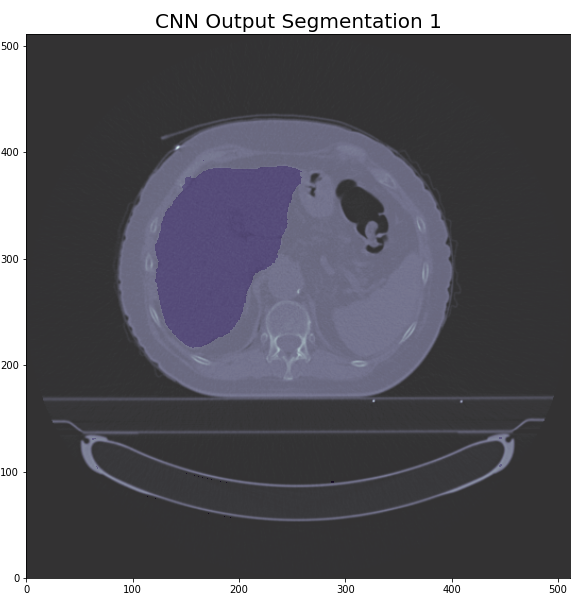
\includegraphics[width=.4\linewidth]{graphics/CNNOutputSegmentation0.png}\label{CNN}}
  \caption{A comparison between the manual segmentation of a CT scan slice and the output of the CNN segmentation.}
  \label{fig:Segmentations}
\end{figure}

\subsection{Calculating the LSN score}

\color{black}
LSN analysis was performed on a selection of the data set. Two lines had to be found. The first, a smooth polynomial line, was found by using an active contour on the 2D binary mask from the segmentation. A section of the boundary could be isolated to calculate the LSN score (Figure \ref{snake}). 
\\ \\
\begin{figure}[h!!]
  \centering
  \subfloat[]{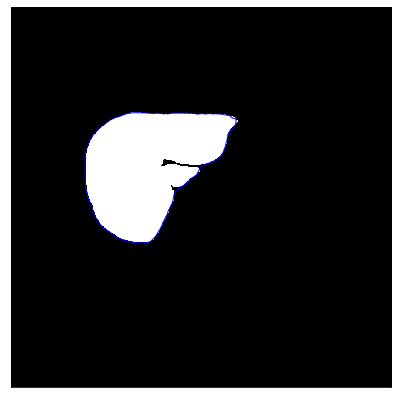
\includegraphics[width=.4\linewidth]{graphics/snake_maskLUNG043.png}\label{snake}}\hspace{1em}
  \subfloat[]{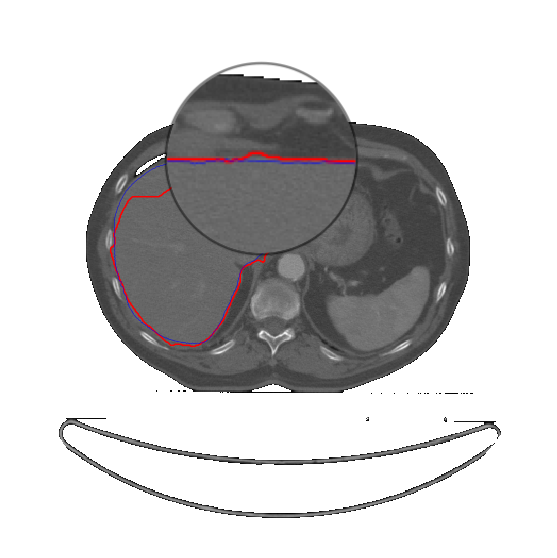
\includegraphics[width=.4\linewidth]{graphics/LUNG043_two_lines.png}\label{two_lines}}
  \caption{Boundaries drawn onto the arrays. Figure \ref{snake} shows a blue polynomial line fit to the segmentation of the liver. Figure \ref{two_lines} shows the true boundary of the liver segmented using a geodesic active contour on top of the blue polynomial lines, and the original CT scan image. The section inside of the circle was used to calculate the LSN score.}
  \label{boundaries}
\end{figure}

The second line used a geodesic active contour find the true boundary of the liver. This consistently found the boundary of the liver, but would sometimes get stuck at seemingly flat sections, as in the top left of Figure \ref{two_lines}. This was also difficult to find for patients who had little fat surrounding their liver. 
\\ \\
Using the two boundaries identified, the LSN was calculated on a section of the liver. This required manual input to identify the most suitable region to use for analysis. This region was one with a clear boundary with fat, usually at the front of the body, at the top of the CT scan. To measure the mean pixel distance between the two segmentations, two lines with the same end points were drawn. The smooth line was drawn using the segmentation, and the second line used the original CT slice image. The distance in terms of pixels was measured for each point on the lines, and the mean was taken giving the LSN value. Having to manually select the coordinates of the end points of the line meant the process could not be fully automated for the whole data set. 
\\ \\
To calculate the error in the value of the LSN, multiple lines were drawn along the boundary with an LSN score calculated for each. In this case, five measurements were taken and a mean was calculated, with the end-points of the line shifted along the liver boundary. The error quoted is the standard deviation of the LSN scores for each line.
\\ \\
Calculating an LSN score from the output of the six test scans for the CNN, a comparison between manual and automatic segmentation was made (Table \ref{tab:comparison}). The LSN scores for automatic segmentation and manual segmentation agree with each other. 
\\ \\
\begin{table}[h]
    \centering
    \caption {Summary table of the six test segmentations. For each case, the LSN value is quoted for both manual and automatic segmentation and the DSC loss value is given.}
    \label{tab:comparison}
    \begin{tabular}{c|c c c}
        Patient ID & LSN score for  & LSN score for & DSC loss value \\
        &auto-segmentation&manual segmentation\\
        \hline
        LUNG1-091 & $1.01\pm 0.14$ &$1.01\pm0.19$&0.0015\\
        LUNG1-092 & $2.54\pm 0.29$ &$2.32\pm0.38$& 0.0053\\
        LUNG1-096 & $2.16\pm0.32$ & $2.20\pm0.32$&0.0022\\
        LUNG1-097 & $2.06\pm0.16$ &$2.08\pm0.12 $&0.0023\\
        LUNG1-099 & $1.52\pm0.21$ &$1.46\pm0.25 $&0.0060\\
        LUNG1-100 & $1.27\pm 0.15$&$1.37\pm0.15$&0.0018
    \end{tabular}
\end{table}

The distribution of LSN scores was found by plotting a histogram for 15 results, Figure \ref{fig:histogram}. While this only shows a small number of patients, the distribution appears to show a trend. Only with clinical data on liver cirrhosis can the LSN score distribution have a definitive boundary between a supposed healthy liver and a cirrhotic liver.

\begin{figure}
    \centering
    
    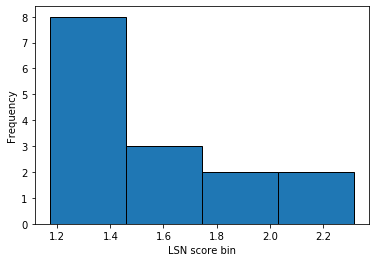
\includegraphics[width=0.8\linewidth]{graphics/histogram.png}
    \caption{Histogram of LSN scores for 15 patients. There is a clustering of patients below LSN of 1.46. Above this could be an indication of cirrhosis. A larger sample of clinical data is needed to make this assessment.}
    %[1.172  1.4585 1.745  2.0315 2.318 ]

    \label{fig:histogram}
\end{figure}
\section{Discussion}
The aim of this project was to produce an automatic tool to assess liver cirrhosis in order to study the relationship between liver cirrhosis and lung cancer. A programme was developed to automatically detect the liver from a patient's lung cancer scan, automatically segment the liver and to evaluate the level of cirrhosis in the liver. This could be used to retrospectively study a large cohort of data. A connection between liver cirrhosis and the treatment of a patient will be of great use in the future for the treatment of lung cancer. 
\\ \\
The study was able to automate individual stages of the process that work as well as the existing manual process. However, the whole process was not able to be automated.  There is still a need for manual input to select the region of the liver for LSN analysis.  Further work in this area could result in the full automation of the process. 
\\ \\
To fully automate the process, first the liver has to be automatically identified in a full CT scan. A review of previous work on liver cirrhosis evaluation has indicated that this has not been achieved in the past and is a new area of research. Two techniques were investigated in identifying a usable CT slice in a patient, and both methods found a usable slice of the liver, but not consistently. However, the idea of finding only one slice of the liver may not be the correct path to follow. Using a well trained neural network, it should be possible to auto-segment any slice of the liver. Combined with a fully automatic method of calculating the LSN score for a slice, a more precise LSN score for a patient may be calculated by using multiple slices from the same CT scan. This would give more confidence in the LSN score, as an average of many slices of the liver would give an LSN of the whole liver, not just one CT slice. By performing small modifications to both methods described previously, multiple slices from the same patient could be automatically selected from a CT scan folder.
\\ \\
To undertake the LSN analysis of patients, a line was fit to the boundary of the liver using an active contour model. The literature that this study is based on does not fully explain their method of calculating the LSN value \cite{Sartoris:2018aa}. There are many sources of error when calculating the LSN score. There is a human error in performing segmentation (that will also transfer into error in the result of the neural network), error in how sharp the CT image is, error in the active contour algorithm. The difficulty in finding a boundary for the liver in patients with little fat also adds error to the effectiveness in using an LSN score for all patients, and is discussed in Goshima and Bae's letter to Radiology \cite{Goshima:2017aa}. The calculation of LSN scores has not been standardised. Thus, the LSN score needs to be a self-consistent metric. The uncertainty of the LSN score is a measure of stability after small changes to the end points of lines. In this case, the error is based on the standard deviation in LSN values range from 6\% to 21\%. This is not as precise as is desirable. 
\\ \\
Automatic segmentation of the liver with the use of a neural network is a method that does not appear in other literature. With a DSC loss value of \hbox{$0.0032\pm0.0018$}, the CNN can automatically segment the liver accurately. The LSN scores from the automated process used were consistent with the scores produced by the manual process. From this successful result, it can be concluded that the CNN in this process can replace the manual input, a step towards full automation. 
\\ \\
Looking at the distribution of LSN scores, there is a cluster below the LSN value of 1.46. This may indicate that above this value a liver is more likely to have cirrhosis, but without performing the analysis on a data set with of known cases of cirrhosis, it is cannot be said definitively. LSN scores are a biomarker for cirrhosis, but more research has to be undertaken before a connection between the LSN value and level of cirrhosis can be confirmed. Research with a clinical data set larger than 15 patients would enable a more precise boundary between a healthy liver and cirrhotic to be identified. A fully automated system would allow for analysis of large data sets.
\\ \\
Further research needs to be undertaken on the relationship between the LSN score to the effects of treatment for lung cancer and to the survival rate of the lung cancer patients. This project looked at the connection between lung cancer and liver cirrhosis, hence why the analysis was performed on data set of lung cancer patients. If found, a link between an LSN score and survival could help in the treatment of these patients. 

\section{Conclusion}
To conclude, a good framework for investigating a connection between lung cancer and liver cirrhosis has been created. By using the methods described to locate the liver based on CT scan folders; using a transfer learning neural network to perform segmentation of the liver and then to perform an LSN analysis on the liver, there is a strong basis for future work in this area. While not fulfilling the initial aim, success in developing a technique to identify the liver in CT scans will be very useful in future work.
\\ \\
Automating the process of calculating the LSN score will allow analysis to take place of large data sets effectively and efficiently. This could be used to identify the LSN scores for cirrhotic livers which would enable detailed investigations into a connection between treatment of lung cancer and liver cirrhosis to be undertaken. This is a new and exciting area of analysis and work should continue to investigate and complete the original aim. 

\cleardoublepage
\bibliographystyle{IEEEtran}
\bibliography{liver.bib}
\end{document}